\ssection{Related Work}
\label{sec:prior}

Several studies have investigated timing side-channels in ReRAM crossbars \cite{kommareddy2019crossbar, khan2021comprehensive, krautter2022data, wang2023side}. These attacks have been evaluated by simulating these asymmetries and demonstrating how they project into various crossbar architectures. Prior investigations do not consider the effects of ECC and how ECC functions may impact crossbar timing measurements. Our results demonstrate the ECC significantly effects the timing of commercial ReRAM crossbar memories. BREW-RC closes this gap by providing a mechanism to derive timing models which incorporate timing perturbations caused by parity bit transitions.

% In this work, we will demonstrate that knowledge of codeword transition DHW $\left( w_{0\to1}, w_{1\to0} \right)$ can accurately predict the distribution of write latencies in commercial memories. However, absent knowledge of the underlying ECC function, the codeword $\left( w_{0\to1}, w_{1\to0} \right)$ becomes ambiguous, complicating timing side-channel attacks. BREW-RC (Section \ref{sec:brew-rc}) closes this gap by extracting the relationship between data bits and parity bits ($P$), allowing both the recovery of critical reliability information, and the generation of more accurate timing models in commercial ReRAM products.

% The AFM paper has no discrepencies with our work. The AFM thesis does. It'll be shorter and easier to just say we are in agreement with their work.
In \cite{tay2023investigation}, atomic force microscopy (AFM) is used to reverse engineer the logical to physical data mapping of the 4M. 
The authors de-layer the device, apply text vectors through the SPI interface, and probe the chip to determine the physical destination of the applied test vectors. 
% Assuming the presence of an ECC function, the minimum hamming distance $D_{min}$ between the reported codewords is 2, an unrealistically low $D_{min}$ for a code rate of $\frac{5}{21}$, as it provides no more error correction than a simple parity check, which can be achieved with a single bit per-word. To check our results against \cite{tay2023investigation}, 
We generate parity bits for the same set of test patterns using $G_{4M}$. We cannot know the correct physical mapping of our extracted parity bits (i.e. the column order of $P$) nor if data was loaded MSB- or LSB-first. Therefore, we compute the minimum distance between our 55 generated parity bits and the 55 parity bits reported in \cite{tay2023investigation} for all possible ($5! * 2$) arrangements and bit orders. 
% % The actual publication drops this specific set of test vectors, so I don't add it into the paper.
%   Our results have no inconsistency with the published paper, only 1 codeword in the published thesis.
\begin{figure}[t!]
    \centering
    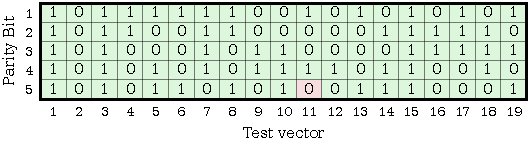
\includegraphics{fig/images/pdf/afm-comparison.pdf}
    \caption{Discrepancy between BREW-RC output and codewords reported in  \cite{tay2023thesisinvestigation}.
    \Description{An 8$\times$21 grid is shown representing the sub-array states of the MB85AS4MT under various test vectors reported in \cite{tay2023thesisinvestigation}. Green grid elements represent consistency with our results. In one location there is an inconsistency.}
    \label{fig:afm-comp}}
\end{figure}
One configuration results in a perfect match between generated codewords and the 55 parity bits reported by the authors, while the next-best configuration has a distance of 18 bits, demonstrating agreement with destructive reverse engineering techniques.
% By fixing this discrepancy, corresponding to test pattern 4, row 8 applied in \cite{tay2023investigation} (see Figure \ref{fig:afm-comp}), all codewords reported by the authors yields a reasonable $D_{min}$ for a rate $\frac{5}{21}$ ECC. We therefore believe this discrepancy to be the result of a transcription or measurement error.

\cite{tolga2024trng} and \cite{suri2018high} use the 4M to implement security primitives. Both papers use $t_w$ as an entropy source. The authors of \cite{tolga2024trng} are able to identify the a latent structure present in $t_w$ measurements but do not identify ECC as the root cause. Instead the authors truncate timing measurements, using the LSB of latency measurements to construct their proposed TRNG. The authors of \cite{suri2018high} initially observe poor PUF performance which is alleviated by effectively hashing two latency measurements using a sum-of-squares technique. Our results indicate that a significant portion of the apparent entropy in 4M/8M latency is structured by hidden ECC activity. Particularly in the 4M, knowledge of the underlying ECC explains nearly all measurement variance. We believe BREW-RC's improved timing model may be useful for improving entropy harvesting by isolating true timing variations from deterministic ECC perturbations.

% The authors note that the MB85AS4MT remains biased under their applied test patterns. Based on our analysis, we attribute this bias to hidden parity bit coupling within the devices on-chip ECC, and we believe a stronger TRNG could be realized by accounting for the full codeword structure and parity dependencies.
% Not really relavant here, this paper has so many
% In \cite{ferdaus2024hiding}, the authors implement a steganographic method to efficiently encode and decode information using the wear-level of bit-cells within the MB85AS4MT. In the context of ECC parity bit coupling, more discrete information encoding techniques may be possible in which the wear-level of ECC bits can be used rather than data bits themselves. Rather than directly hammering repeated patterns (a practice which is easily detectable in modern systems) 